% Q8 原图几何关系的空间示意；不表示各边实际比例。
% 构形：BD=2，C=(1,sqrt(3),0)，A=(1,0,1)，仅用于满足题设关系。
% right angle: BAD; midpoint: E on BC; perpendicular planes: (ABD) and (BCD).
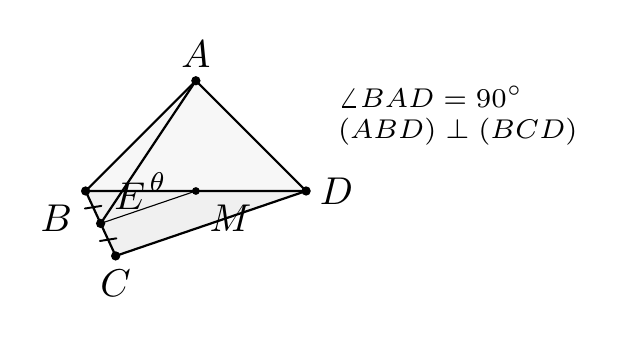
\begin{tikzpicture}[scale=1.4,transform shape,
  x={(1cm,0cm)}, y={(-0.42cm,-0.34cm)}, z={(0cm,1cm)},
  line cap=round, line join=round, >=stealth
]
  \coordinate (B) at (0,0,0);
  \coordinate (D) at (2,0,0);
  \coordinate (C) at (1,1.732,0);
  \coordinate (A) at (1,0,1);
  \coordinate (E) at (0.5,0.866,0);
  \coordinate (M) at (1,0,0);

  % The two triangles lie in perpendicular planes and share BD.
  \fill[black!3] (B)--(D)--(A)--cycle;
  \fill[black!6] (B)--(C)--(D)--cycle;
  \draw[thick] (A)--(B)--(D)--cycle;
  \draw[thick] (B)--(C)--(D);
  \draw[thick] (A)--(E);
  \draw[thin] (M)--(E);

  % E is the midpoint of BC; M is the midpoint of BD and the foot of A.
  \fill (A) circle (1.2pt) node[above] {$A$};
  \fill (B) circle (1.2pt) node[below left] {$B$};
  \fill (C) circle (1.2pt) node[below] {$C$};
  \fill (D) circle (1.2pt) node[right] {$D$};
  \fill (E) circle (1.2pt) node[above right] {$E$};
  \fill (M) circle (1pt) node[below right] {$M$};

  % Short matching ticks on BE and EC indicate the stated midpoint.
  \draw[line width=0.7pt] (0.31,0.398,0) -- (0.19,0.468,0);
  \draw[line width=0.7pt] (0.81,1.264,0) -- (0.69,1.334,0);

  \node[align=left,anchor=west,font=\scriptsize] at (2.25,0.20,0.75)
    {$\angle BAD=90^\circ$\\$(ABD)\perp(BCD)$};
  \node[font=\scriptsize] at (0.70,0.12,0.12) {$\theta$};
\end{tikzpicture}
